\chapter{Bring your own Device (BYOD)}
In today's business, many employees want to work on their own device. Whether it is to be mobile or just to have more familiarity to the platform used, the employer has to react to this trend. There are many reasons for employees to use their own device. Those include for example an increased level of comfort, the proficiency with only one device and the use of mobile devices in the first place. \\
The increased level in comfort comes from the familiarity with the devices the employee uses due to the fact that they use the same device privately as well as at work. And since many people are always online with any device it is possible to work anywhere and anytime instead of being bound to the office and fix work hours. \\
In many companies not every employee is entitled to receive a mobile device for work. Only those with a certain position, where it is needed to be able to work on the go. With BYOD it is possible for every other employee to work on their own mobile device instead. Which in turn can increase their productivity, customize their working hours and give freedom for their work place.\\


\section{Device Provisioning}
There are different strategies to provide Devices for the employees. Each varies in enterprise control and Employee Satisfaction. The strategies can be divided into 4 concepts. \parencite{KumarGajar.2013}
\begin{enumerate}
	\item Here's your own Device (HYOD) \\
	With this concept the company decides on everything regarding the device. From the buying process over the installation, configuration and support to the disposal of the device, everything is managed by the company, giving full control and oversight over the life cycle of every device. Whereas the employees has no control except for minor customization options and applications.  \parencite{KumarGajar.2013}
	
	\item Choose your own Device (CYOD) \\
	This approach gives the employee some choice for the device he gets from the company. The company gives the employee a selection of different pre-chosen devices. This gives some options when it comes to manufacturer, operating system and hardware specifications. The pre-selection as well as installation and set-up are still responsibilities of the company. The support is more complicated, since the IT help desk needs to be proficient with all offered equipment. Company-wide software also needs to run on every device which leads to higher implementation overhead and costs. \parencite{KumarGajar.2013}
	
	\item Bring your own Device (BYOD) \\
	Bring your own Device is the concept of using existing private devices in a work environment. Alternatively the company can provides financial help for the employee to buy a device. This allows the employee to freely choose the device, like operating system, manufacturer and hardware specification. This also includes the type, i.e. Desktop Computer, Laptop, Workstation, Tablet, Smartphone, of the device. If he wants to, he can also use multiple different devices. Since the device is owned by the employee, he has most control over it. However, the company can introduce policies since the employee works with (often confidential) company data. Support can often only be provided on a basic level, since every employee can have a different device and to provide expertise for all of them is too expensive to be economical. \parencite{KumarGajar.2013}
	
	\item On your own Device (OYOD) \\
	On your own Device takes it a step further and gives Employees all the freedom he can get. Not even Policies are put in place by the company, making it the option with highest employee satisfaction, but with the lowest enterprise control. \parencite{KumarGajar.2013}
\end{enumerate}
These 4 concepts are not a strict representation of all possibilities. For example, it is possible to give the employee a choice of operating system, while having only one device. This combines both HYOD and CYOD. That's why every company should consider BYOD besides their current strategy, enabling employees to use their own devices alongside any other device. Chances are they are already using it despite it being not officially supported or even allowed. \parencite{IBMSecurity.2016}. But with no BYOD policies in place it is more like OYOD. As seen in the figure \ref{fig:control_v_satisfaction} below, OYOD does not allow any control over the device, which makes it a potential security issue.
\begin{figure}[H]
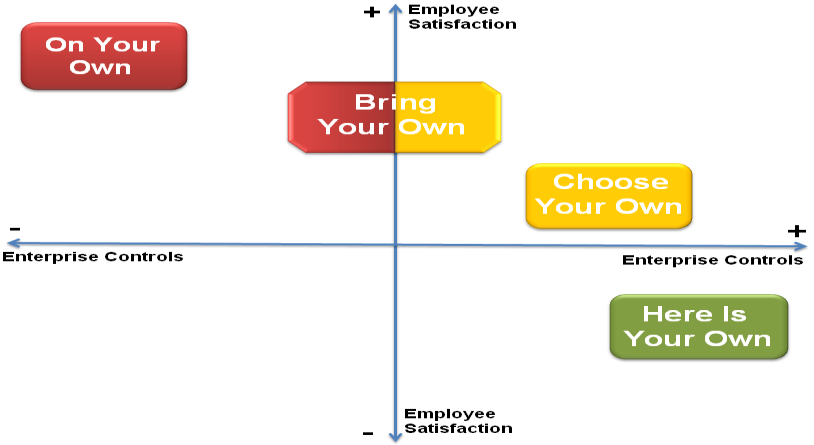
\includegraphics[width=0.7\linewidth]{images/control_v_satisfaction}
\caption{Enterprise Control and Employee Satisfaction of provision strategies \parencite{KumarGajar.2013}}
\label{fig:control_v_satisfaction}
\end{figure}

\section{Architectural Concepts}
There are different technological approaches for using BYOD in a company. Figure \ref{fig:architectural_concepts} shows how company applications can be used from an end user device. The different approaches are compared between presentation, application execution, application launch and data storage. While most of the approaches do not need to store the data on the device, it can be done to optimize network or hardware usage \parencite{Disterer.2013}
\begin{figure}[H]
	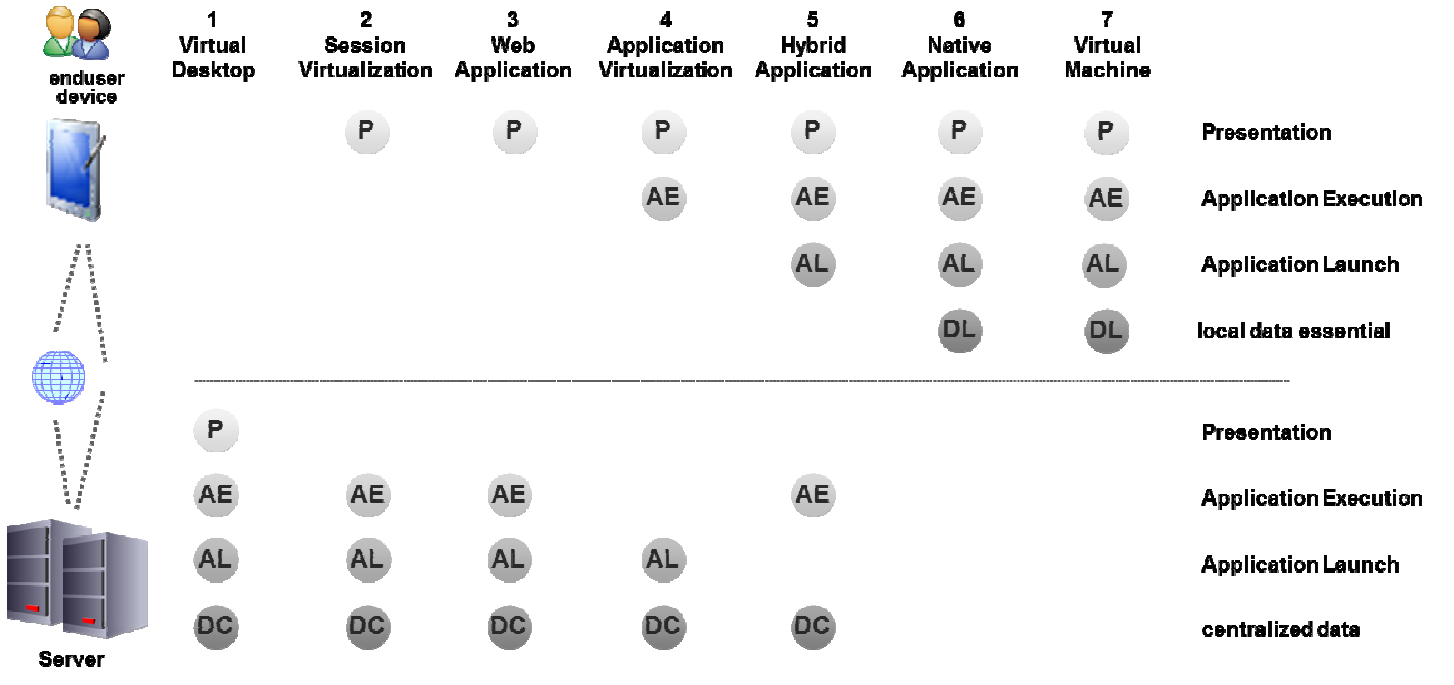
\includegraphics[width=1\linewidth]{images/architectural_concepts}
	\caption{Architectural Concepts and Technological Approaches \parencite{Disterer.2013}}
	\label{fig:architectural_concepts}
\end{figure}
\begin{enumerate}
	\item Virtual Desktop \\
	The employee device launches a virtual machine on a server in the company's network. Every part of the application runs on the server, even the presentation. This makes it the mobile equivalent to a terminal server. As with terminals, all the information for the presentation and user input is sent over the network. However, with a stationary terminal bandwidth is not such a big problem as with mobile devices, which makes this approach not feasible for the time being.  \parencite{Disterer.2013}
	\item Session Virtualization \\
	In \textit{session virtualization}, the client also starts an application on a server in the company's network. The execution and data storage is all done by the server, but the user interface is created on the client device. This reduces the bandwidth, since the client does not need as much information to create the user interface as the \textit{virtual desktop} does to provide the interface itself. Since the end user device creates the interface, the look \& feel and the control scheme can be device specific. This however requires additional implementation effort for each device. \parencite{Disterer.2013}
	\item Web Application \\
	With pure HTML \& CSS this is a special kind of \textit{session virtualization}. If the HTML is extended by JavaScript or some enhanced HTML5 functions, this is considered a \textit{Hybrid Application} instead of a \textit{session virtualization}. Nowadays \textit{web applications} are widely used in many areas. There is a great number of implementations of the standard. For virtually every device there is a browser, which can display the information from the web server. Compared to \textit{virtual desktops} and other \textit{session virtualizations} the bandwidth used is low, making it a better solution for mobile devices. \\
	While the use of a standardized solution is a big advantage for the most part, it also can have disadvantages. For example there is more malware for widely spread software. Another disadvantage is that modern browser access the local system and store potentially confidential data on the device, which poses a security risk. \parencite{Disterer.2013}
	\item Application Virtualization \\
	As seen in Figure \ref{fig:appVirtual} below, in \textit{Application Virtualization} the applications run in an emulator instead of just on top of the operating system. The functions of the operating system are emulated for the application. \parencite{Husain.2008} This has the advantage that the application does not have to be developed for multiple systems. If a new system gets released or an old system gets updated, the developers only need to change the emulator but not all the applications that are supposed to run on that system. With this approach applications often run in separate sandboxes/containers. The applications therefore are isolated from other software running on the device. This reduces the risk of another software interfering with the application as well as preventing it from accessing personal data on the device. \parencite{Disterer.2013}
	\begin{figure}[H]
		\includegraphics[width=1\linewidth]{images/appVirtual}
		\caption{Application running in a native environment and an application virtualization environment \parencite{Egmason.2011}}
		\label{fig:appVirtual}
	\end{figure}
	\item Hybrid Application \\
	\textit{Hybrid Applications} combine \textit{Session Virtualization} with \textit{Native Applications}. The most widespread example are web applications. Locally JavaScript and HTML can execute some parts of the application and the other part is executed on the web server. For the most part \textit{hybrid applications} should be considered as \textit{native applications} when it comes to security  \parencite{Disterer.2013}
	\item Native Application \\
	 \parencite{Disterer.2013}
	\item Virtual Machine \\
	 \parencite{Disterer.2013}
\end{enumerate}

\section{Disadvantages}

\section{Risks}
